\begin{figure}[H]
\centering
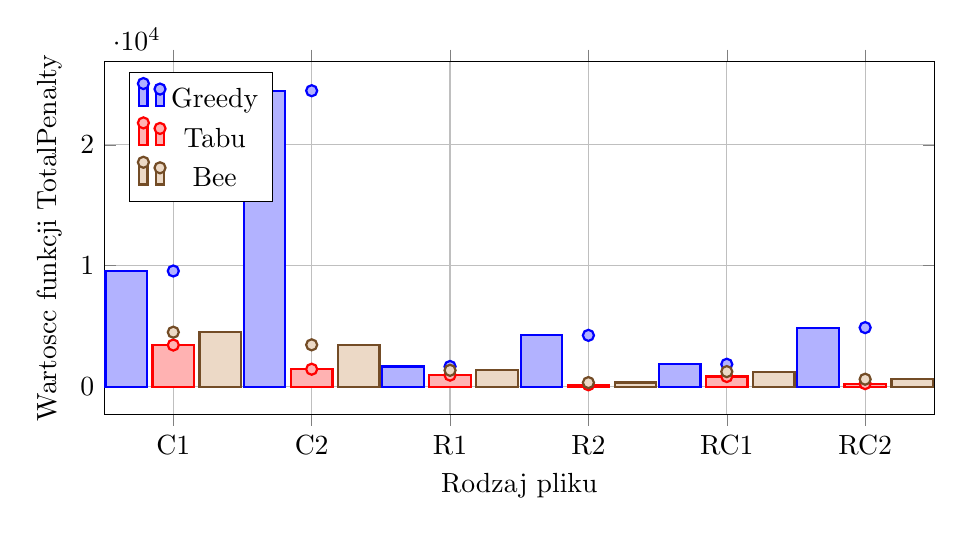
\begin{tikzpicture}
\begin{axis}[
xlabel = {Rodzaj pliku},
ylabel = {Wartoscc funkcji TotalPenalty},
legend pos = north west,
grid = both,
width=1\linewidth,
height=0.5\linewidth,
ybar,
bar width=15pt,
symbolic x coords={C1,C2,R1,R2,RC1,RC2,},
xtick=data
]
\addplot + [mark = *, thick] coordinates
    {
(C1,9566.777777777777)(C2,24480.0)(R1,1666.8333333333333)(R2,4242.727272727273)(RC1,1850.0)(RC2,4881.375)};
\addlegendentry
{Greedy}
\addplot + [mark = *, thick] coordinates
    {
(C1,3439.0)(C2,1438.875)(R1,950.8333333333334)(R2,151.8181818181818)(RC1,834.5)(RC2,245.125)};
\addlegendentry
{Tabu}
\addplot + [mark = *, thick] coordinates
    {
(C1,4502.666666666667)(C2,3456.625)(R1,1349.0)(R2,332.6363636363636)(RC1,1241.5)(RC2,612.875)};
\addlegendentry
{Bee}
\end{axis}
\end{tikzpicture}
\caption
{Porownanie srednich wartosci TotalPenalty algorytmow dla kazdego rodzaju pliku}
\label{fig:mean_TotalPenalty_comparision}
\end{figure}
